\documentclass[fleqn]{article}[12pt]

\usepackage{amsmath}
\usepackage{amssymb}
\usepackage{pgfplots}
\usepackage[margin=1in]{geometry}
\usepackage{fancyhdr}
\usepackage{lastpage}
\usepackage{siunitx}
\usepackage{amsthm}
\usepackage{booktabs}


\setlength\parindent{0pt}

\cfoot{\thepage \hspace{1pt} / \pageref{LastPage}}
\newcommand{\integral}[4]{\int_#1^#2 \! #3 \, \mathrm{d}#4}
\newcommand{\dif}{\mathrm{d}}
\newcommand{\diracraw}{\left(\int_{-\infty}^{\infty} e^{i2\pi (f - \bar f)}\, dt\right)}
\usepackage{caption}
\captionsetup{justification=raggedright,singlelinecheck=false}
\DeclareMathOperator{\Imag}{Im}


\DeclareSIUnit\year{yr}
\DeclareSIUnit{\calorie}{cal}

\pgfplotsset{compat=1.14}

\newcommand{\M}{\mathbb{M}}
\newcommand{\W}{\mathbb{W}}
\newcommand{\R}{\mathbb{R}}


\begin{document}
    \begin{tabular}{l}
        ID \#33 \\
        Problem Set 14 \\
        Physics 202 \\
        \today
    \end{tabular}

\begin{enumerate}
    \item Since the amount of gas does not change, $Nk_B$ is constant. Then the initial volume is given by
    \begin{equation*}
        V_i = \frac{Nk_B T}{P_1} = \frac{Nk_B(\SI{626}{\kelvin})}{\SI{1.7e7}{\pascal}}
    \end{equation*}
    and the output volume is
    \begin{equation*}
        V_0 = \frac{Nk_B T}{P_2} = \frac{Nk_B(\SI{323}{\kelvin})}{\SI{10000}{\pascal}}
    \end{equation*}
    The ratio of the volumes is therefore
    \begin{equation*}
        \frac{V_o}{V_i} = \frac{\frac{Nk_B(\SI{626}{\kelvin})}{\SI{1.7e7}{\pascal}}}{\frac{Nk_B(\SI{323}{\kelvin})}{\SI{10000}{\pascal}}} =
        0.00114
    \end{equation*}
    The total amount of gas per second is $\SI{400}{\kg/s} \times \SI{1000}{\g/\kg} / \SI{18.01}{\g/\mol} = \SI{22209}{\mol/\s}$. Then
    \begin{equation*}
        E_{th,i} = 3 Nk_B T = 3 (\SI{8.314}{\joule/\mol\kelvin})(\SI{22209}{\mol/\s}) (\SI{626}{\kelvin}) = \SI{3.47e8}{\joule/\s}
    \end{equation*}
    and
    \begin{equation*}
        E_{th,f} = 3 Nk_B T = 3 (\SI{8.314}{\joule/\mol\kelvin})(\SI{22209}{\mol/\s}) (\SI{323}{\kelvin}) = \SI{1.79e8}{\joule/\s}
    \end{equation*}
    If all the thermal energy lost is converted into work, the plant outputs
    \begin{equation*}
        \SI{3.47e8}{\joule/\s} - \SI{1.79e8}{\joule/\s} = \SI{1.79e8}{\joule/\s}
    \end{equation*}

    \item Like with the heat engine example in class or in the textbook, the most efficient possible refrigerator uses the Carnot cycle. The work input is part of the two isothermal processes.

    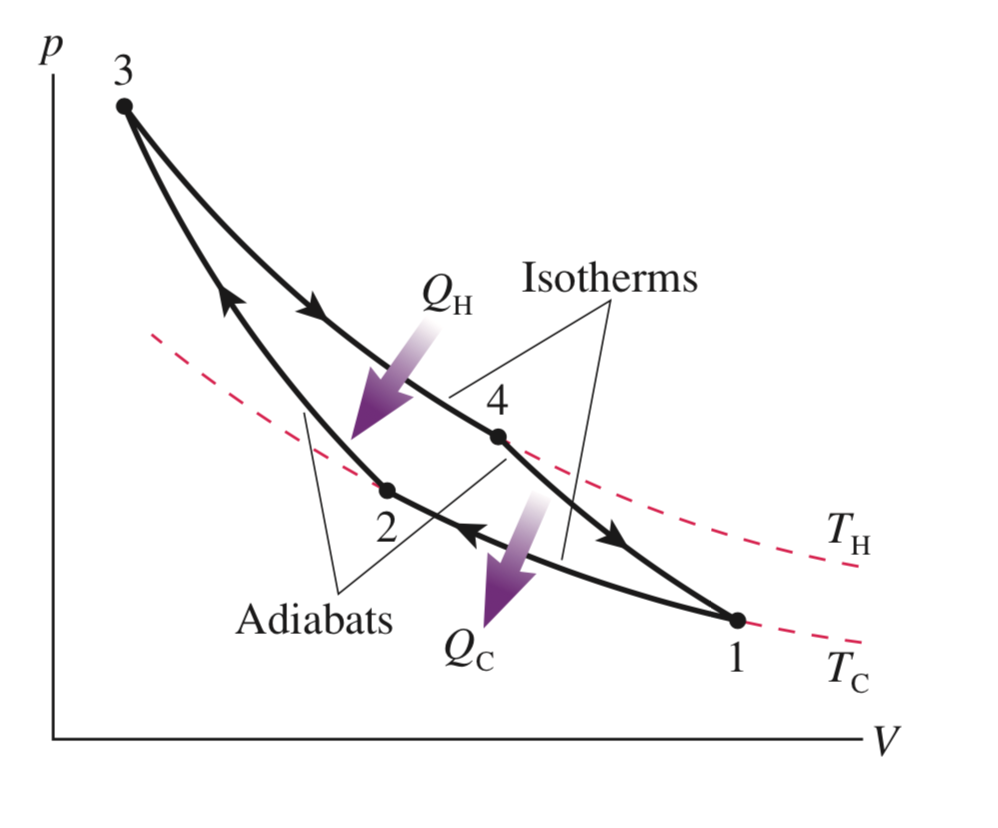
\includegraphics[width=0.4\textwidth]{carnot}

    The cycle diagram for the most efficient refrigerator is like this one, but with the arrows reversed (diagram from the Knight textbook).

    Since the thermal efficiency of any refrigerator is
    \begin{equation*}
        K = \frac{Q_H}{Q_H-Q_C}
    \end{equation*}
    we can figure out the optimal case by calculating the heat transfer for the isothermal processes in the diagram above. Going from position 2 to 1, the heat transfer is
    \begin{equation*}
        Q_{C} = |Nk_BT_C \log(V_1/V_2)|
    \end{equation*}
    The heat transfer from 4 to 3 is similarly
    \begin{equation*}
        Q_{H} = |Nk_BT_H \log(V_4/V_3)|
    \end{equation*}
    so therefore
    \begin{equation*}
        K = \frac{Nk_BT_H \log(V_4/V_3)}{Nk_BT_H \log(V_4/V_3) - Nk_BT_C \log(V_1/V_2)} = \frac{T_H \log(V_4/V_3)}{T_H \log(V_4/V_3) - T_C \log(V_1/V_2)}
    \end{equation*}
    However, for the adiabatic processes,
    \begin{equation*}
        V_2 = V_3\left(\frac{T_H}{T_C}\right)^{1/(\gamma-1)} \qquad V_1 = V_4\left(\frac{T_H}{T_C}\right)^{1/(\gamma-1)}
    \end{equation*}
    so that
    \begin{equation*}
        \frac{V_1}{V_2} = \frac{V_4}{V_4}
    \end{equation*}
    and
    \begin{equation*}
        K_{\text{max}} = \frac{T_H}{T_H-T_C}
    \end{equation*}

    \item \begin{enumerate}

        \item

        \vspace{5cm}
        This cycle can be used as a heat engine, but not as a refrigerator because a refrigerator requires adiabatic compression and expansion steps, and this cycle only has an adiabatic expansion.

        \item The work output of one cycle is equal to the area inside the cycle. To calculate that, we first need functions for each of the three processes:
        \begin{align*}
            &P_{1-2}(V) = P_1 \\
            &P_{2-3}(V) = \frac{C_1}{V^\gamma} = \frac{P_1V_2^\gamma}{V^\gamma} \\
            &P_{3-1}(V) = \frac{C_2}{V} = \frac{P_1V_1}{V}
        \end{align*}
        The last component we need is the volume at point 3. Setting the adiabat and isotherm equal and solving for $V$ gives
        \begin{equation*}
            V_3 = \left(\frac{V_2^\gamma}{V_1}\right)^{1/(\gamma-1)}
        \end{equation*}
        Then the work is
        \begin{align*}
            W &= \int_{V_1}^{V_2} P_{1-2}(V) dV + \int_{V_2}^{V_3} P_{2-3}(V) dV + \int_{V_3}^{V_1} P_{3-1}(V) dV  \\
            &= \int_{V_1}^{V_2} P_1 dV
                + \int_{V_2}^{\left(\frac{V_2^\gamma}{V_1}\right)^{1/(\gamma-1)}} \frac{P_1V_2^\gamma}{V^\gamma} dV
                + \int_{\left(\frac{V_2^\gamma}{V_1}\right)^{1/(\gamma-1)}}^{V_1} \frac{P_1V_1}{V} dV \\
            &= \left(\left.
                PV
            \right|_{V=V_1}^{V_2}\right) +
            \left(\left.
                \frac{P_1 V^{1-\lambda} V_2^\lambda}{1-\lambda}
            \right|_{V=V_2}^{\left(\frac{V_2^\gamma}{V_1}\right)^{1/(\gamma-1)}}\right) +
            \left(\left.
                P_1V_1\log(V)
            \right|_{V=\left(\frac{V_2^\gamma}{V_1}\right)^{1/(\gamma-1)}}^{V_1}\right) \\
            &= P_1 \left(-\frac{V_2^{\lambda} \left(\left(\frac{V_2^{\lambda}}{V_1}\right)^{\frac{1}{\lambda-1}}\right)^{1-\lambda}}{\lambda-1}-V_1 \log \left(\left(\frac{V_2^{\lambda}}{V_1}\right)^{\frac{1}{\lambda-1}}\right)+\frac{V_2}{\lambda-1}-V_1+V_1 \log (V_1)+V_2\right)
        \end{align*}

        \item The efficiency is given by
        \begin{equation*}
            \eta = \frac{W}{Q_H} = \frac{P_1 \left(-\frac{V_2^{\lambda} \left(\left(\frac{V_2^{\lambda}}{V_1}\right)^{\frac{1}{\lambda-1}}\right)^{1-\lambda}}{\lambda-1}-V_1 \log \left(\left(\frac{V_2^{\lambda}}{V_1}\right)^{\frac{1}{\lambda-1}}\right)+\frac{V_2}{\lambda-1}-V_1+V_1 \log (V_1)+V_2\right)}{n C_P \log(V_2/V_1)}
        \end{equation*}
    \end{enumerate}

    \item \begin{enumerate}
        \item Rewriting van der Waals' equation as a function of $V$ gives that
        \begin{equation*}
            P(V) = \frac{a b n-a V+b n^3-n^2 V+n R T V^2}{V^2 (V-b n)}
        \end{equation*}
        The work done on a gas undergoing a volume change from $V_1$ to $V_2$ is
        \begin{equation*}
            \int_{V_1}^{V_2} \frac{a b n-a V+b n^3-n^2 V+n R T V^2}{V^2 (V-b n)} dV =
            nRT\log((V_2-bn)/(V_1-bn)) + \frac{a n^2 (V_1-V_2)}{V_1 V_2}
        \end{equation*}
        When $a=0,b=0$,
        \begin{equation*}
            W =
            nRT \log\left(\frac{V_2}{V_1}\right)
        \end{equation*}

        \item In the ideal gas case, the work done is
        \begin{equation*}
            W_{\text{ideal}} = n R T \log(V_2/V_1) = (\SI{1}{\mol})(\SI{8.314}{\joule/\mol\kelvin})({\SI{293}{\kelvin}}) \log(0.5) = \SI{1688}{\joule}
        \end{equation*}
        In the nonideal case, the work is
        \begin{align*}
            &W_{vdW} = nRT\log((V_2-bn)/(V_1-bn)) + \frac{a n^2 (V_1-V_2)}{V_1 V_2} \\ &=
            (\SI{1}{\mol})(\SI{8.314}{\joule/\mol\kelvin})({\SI{293}{\kelvin}}) \log\left(
                \frac{\SI{0.0112}{\m^3}-\SI{23.71e-6}{\m^3}}{\SI{0.0224}{\m^3}-\SI{23.71e-6}{\m^3}}
            \right) \\
            &+ \frac{\left((\SI{3.46e-3}{\pascal\m^6})(\SI{0.0122}{\m^3})\right)}{\SI{0.000251}{\m^6}} = \SI{1691}{\joule}
        \end{align*}
        Then
        \begin{equation*}
            \Delta W = \SI{3}{\joule},\qquad  \frac{\Delta W}{W_{\text{ideal}}} = \SI{0.00178} = 0.178\%
        \end{equation*}
    \end{enumerate}
\end{enumerate}


\end{document}
